Below is a figure showing the \textbf{empirical pseudo-regret} of two UCB algorithms: ``original UCB'' (red) vs. ``modified UCB'' (blue), for three different gap values \( \Delta = 0.25, 0.125, \) and \( 0.0625 \). Each curve is the average over 20 runs of length \( T=100000 \), with shaded \( \pm1 \) standard-deviation bands.

\begin{figure}[h]
    \centering
    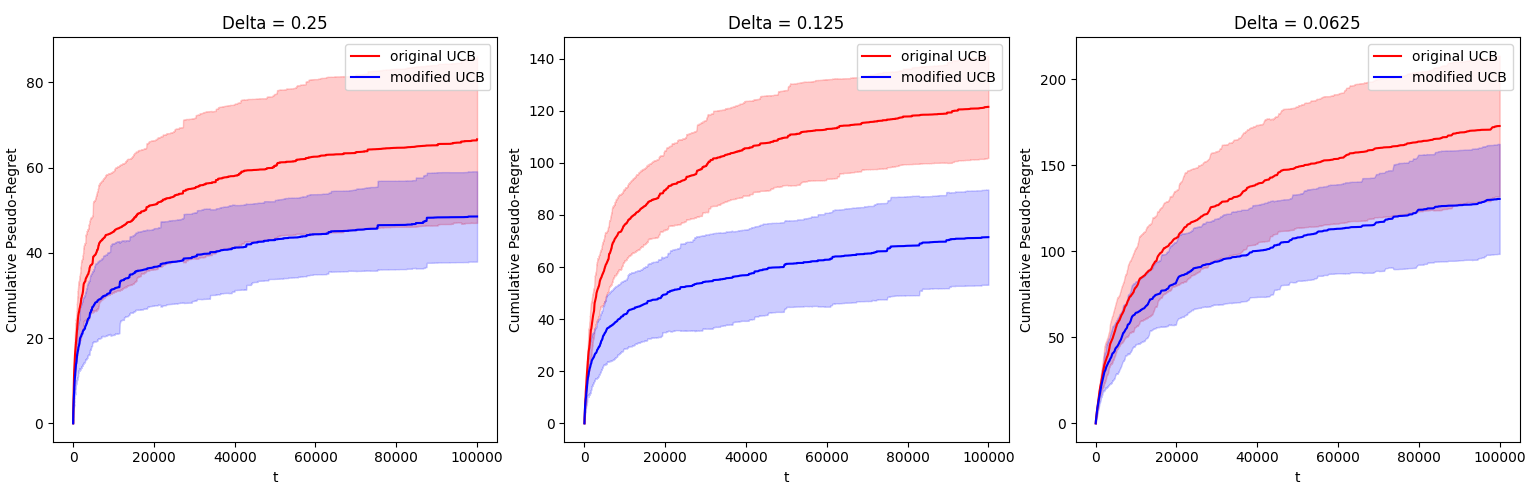
\includegraphics[width=\textwidth]{plots.png}
    \caption{Empirical pseudo-regret over time for different values of \( \Delta \).}
\end{figure}

\subsection{Plot Description}

\begin{itemize}
    \item \textbf{Horizontal axis}: time \( t\in\{1,\dots,100000\} \).
    \item \textbf{Vertical axis}: cumulative pseudo-regret \( \widehat{R}_t \), i.e. \( \sum_{s=1}^t\Delta(A_s) \), where \( \Delta(A_s) \) is the gap between the chosen arm’s mean and the optimal arm’s mean at time \( s \).
    \item \textbf{Subplots}: from left to right, we show the same experiment but with \( \Delta=0.25,\ 0.125,\ \text{and}\ 0.0625 \).
\end{itemize}

In all three cases, the \textbf{blue (modified UCB)} curve remains below the \textbf{red (original UCB)} curve, indicating the modified parametrization typically achieves lower pseudo-regret. We also see that for smaller \( \Delta \) (rightmost plot), overall regret magnitudes are higher.

\subsection{1) Which values of \( \Delta \) lead to higher regret?}

We see from the three subplots that:
\begin{itemize}
    \item \( \Delta=0.25 \) (left) yields smaller final regrets, on the order of \( \approx 60 \) for the original UCB and \( \approx 40 \) for the modified UCB by \( t=100000 \).
    \item \( \Delta=0.125 \) (middle) has higher final regret (\( \approx 120 \) vs. \( \approx 60 \)).
    \item \( \Delta=0.0625 \) (right) yields still higher regrets (\( \approx 170 \) vs. \( \approx 120 \)).
\end{itemize}

Hence, \textbf{the smaller \( \Delta \) is, the higher the pseudo-regret} tends to be. Intuitively, when the arms’ means are closer together, it is harder to distinguish the optimal arm from the suboptimal arm; more exploration is needed before we can reliably exploit.

\subsection{2) Relative performance of the two parametrizations}

Throughout the plots, the \textbf{modified UCB} (blue) consistently achieves lower pseudo-regret than the \textbf{original UCB} (red), with the difference becoming more pronounced over time. This matches the theoretical expectation that using a confidence term of \( \sqrt{\ln t} \) instead of \( \sqrt{\ln t^3} \) results in a tighter exploration bonus, leading to better performance.

The key difference is that the modified parametrization adjusts the confidence radius more efficiently, reducing excessive exploration while still maintaining sufficient uncertainty control. As a result:

\begin{itemize}
    \item \textbf{Modified UCB} adapts the confidence intervals in a way that prioritizes more selective exploration, leading to \textbf{lower regret}.
    \item \textbf{Original UCB} uses a slightly larger confidence bound, which results in more cautious exploration and higher cumulative regret over time.
\end{itemize}

Overall, the modified parametrization demonstrates superior performance across all tested gap values.
